\chapter{Sequence Context Effect}\label{sce}

Different cancers develop under the influence of different conditions, especially mutagens and repair systems, thus each cancer type possesses a distinctive mutation composition. Regarding individual mutation, each base change is closely integrated with the bases next to it \citep{Zhu2017,Zhu2020,Vinson2012CGMethylation}. The question is whether flanking bases beyond 3-mers, specifically positions -2 \& +2, have an influence on whether the mutations occur. Using a measure of information richness, \gls{re}, this chapter demonstrates the importance of both the composition of base changes and their flanking bases in characterising the carcinogenesis pattern, with evidence of strand symmetry. Above all, the chapter shows that the \gls{sce} is not just contributed by immediate flanking bases (\textit{i.e.} 3-mers). Rather, there is certain value in factoring larger sequence contexts into analysing cancer mutation composition.

\section{Base substitutions are indicative of cancers}
SCE consists of two components, the middle base substitutions and the flanking bases. This section focuses on the first component.

\subsection{Base substitutions are a rich source of information}
To explore the patterns of base substitutions and its potential contribution to SCE, I calculated $RE$'s for each mutation of every cancer. $RE$'s are essentially the information which the null cannot capture. Here, the null assumed that all mutations with the same wildtype occurred at the same rates (details in \ref{methods:re}). I plotted $RE$ as sequence logos in Figures \ref{fig:spectra} and \ref{fig:apdx_spectra}, where the height of the letter is the $RE$ of the mutation and its orientation dictates whether the mutation is in excess (up) or deficit (down). We are interested in the shape of the sequence logos. Three features stand out from the plots. First, base substitutions were strand symmetric for all cancers because the plots are point symmetric. That is, $RE$'s are similar for reverse complementary mutations (\textit{e.g.} C$\rightarrow$T and G$\rightarrow$A). Second, the heights of the up-oriented letters for transitions signifies that they were more abundant than transversions. Third, by visualisation, the patterns of base substitutions were very diverse. For example, Skin-Melanoma were predominated by C$\rightarrow$T, but this was not necessarily true in other cancers, such as Liver-HCC. Indeed, Liver-HCC was more strongly0 characterised by the A$\rightarrow$G transitions.

\begin{figure}[ht!]
    \begin{subfigure}{.5\textwidth}
    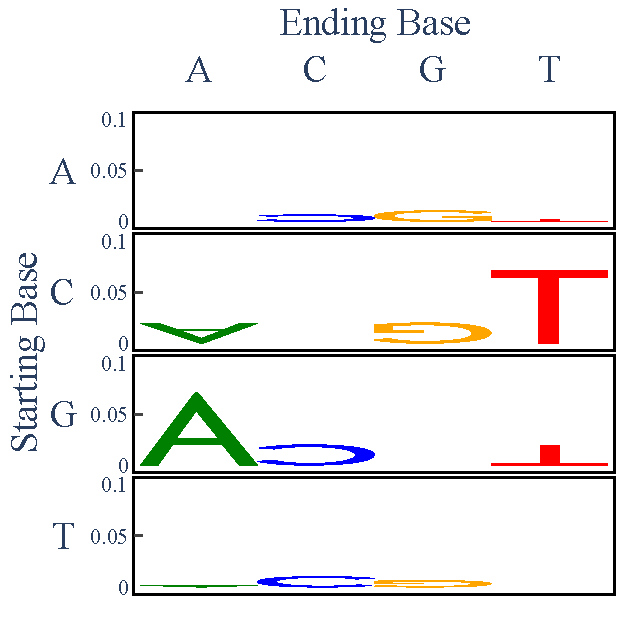
\includegraphics[scale=0.7]{graphics/spectra_Skin-Melanoma.pdf}
    \caption{Skin-Melanoma}
    \label{fig:spectra_skin}
    \end{subfigure}
    ~
    \begin{subfigure}{.5\textwidth}
    
    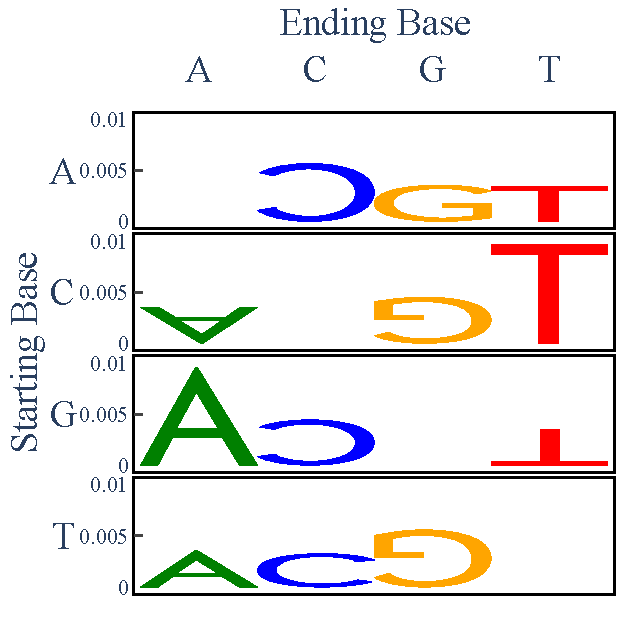
\includegraphics[scale=0.7]{graphics/spectra_Kidney-RCC.pdf}
    \caption{Kidney-RCC}
    \label{fig:spectra_kidney}
    \end{subfigure} \\
    \vspace{0.5cm}
    
    \begin{subfigure}{.5\textwidth}
    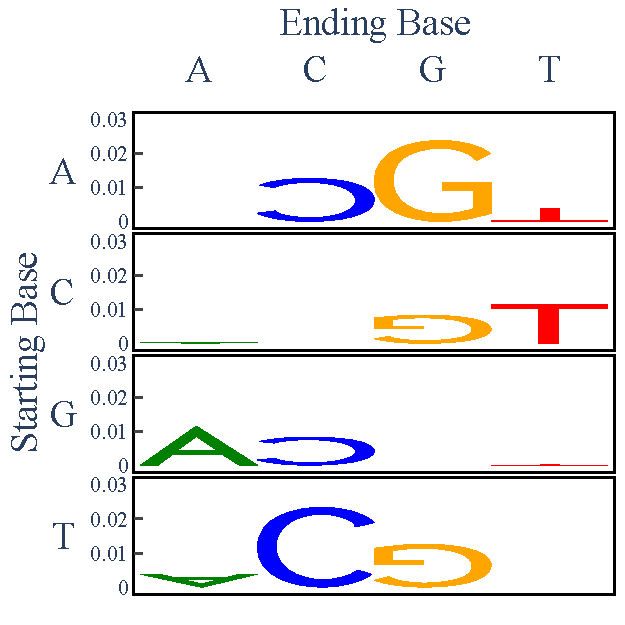
\includegraphics[scale=0.7]{graphics/spectra_Liver-HCC.pdf}
    \caption{Liver-HCC}
    \label{fig:spectra_liver}
    \end{subfigure}
    ~
    \begin{subfigure}{.5\textwidth}
    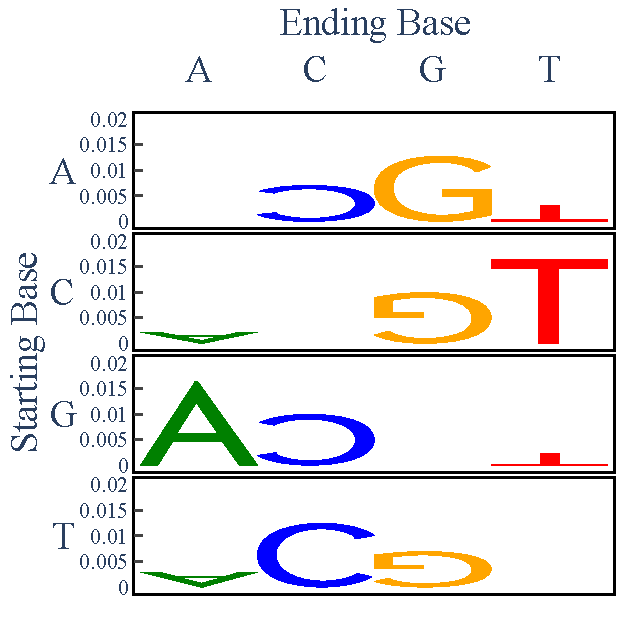
\includegraphics[scale=0.7]{graphics/spectra_Panc-AdenoCA.pdf}
    \caption{Panc-AdenoCA}
    \label{fig:spectra_panc_adenoca}
    \end{subfigure} \\
    \vspace{0.2cm}
    \caption{\textbf{Base substitutions are a rich source of information}. Here, $RE$'s as a measure of information are shown in mutation logos for (a) Skin-Melanoma (b) Kidney-RCC (c) Liver-HCC (d) Panc-AdenoCA. The other cancers can be found in Figure \ref{fig:apdx_spectra}. For each panel, each row was derived from a pair of GLMs corresponding to a wildtype base. The x-axis is the wildtype base; the y-axis is the product of the substitution. The heights of the letters are $RE$'s. An up-orientation indicates an excess while a down-orientation indicates a deficit of the mutation.}
    \label{fig:spectra}
\end{figure}

\subsection{Base substitutions differ in different cancers}
To further confirm that base substitutions could distinguish cancers, I performed a hypothesis test for difference between each cancer pair. One such hypothesis test was an aggregation of 4 GLM, each corresponding to a wildtype base. The 4 p-values from GLM were combined by Fisher's method to obtain a single joint p-value. All pairwise comparisons were statistically significant, with the highest p-value coming from comparing CNS-Medullo with CNS-PiloAstro at 0.0095 after Bonferroni correction. Figure \ref{fig:paired_spectra} demonstrates how individual substitutions could contribute to the whole information content of the test. It is no surprise that in Figure \ref{fig:spectra_kidney_skin}, there was a deficit in C$\rightarrow$T/G$\rightarrow$A in Kidney-RCC with respect to Skin-Melanoma, as we have seen previously that the abundance of C$\rightarrow$T/G$\rightarrow$A was somewhat one ``signature'' of Skin-Melanoma. The same can be said about A$\rightarrow$G/T$\rightarrow$C when comparing Kidney-RCC to Liver-HCC (Figure \ref{fig:spectra_kidney_liver}).

\begin{figure}[ht!]
    \begin{subfigure}{.5\textwidth}
    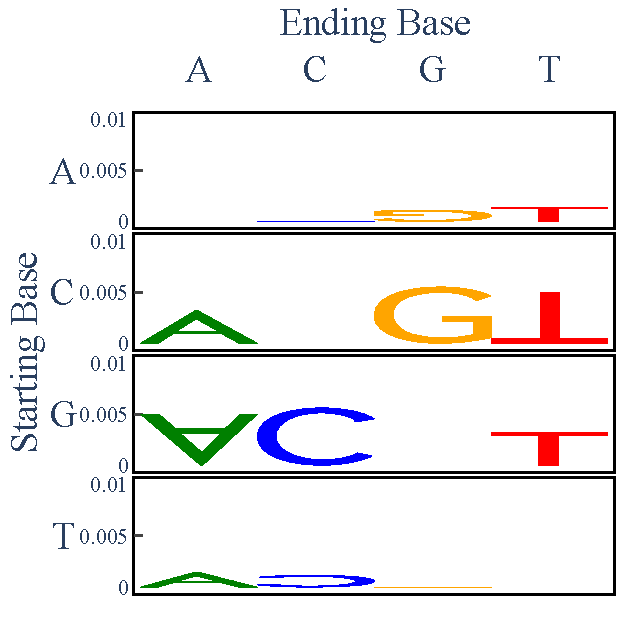
\includegraphics[scale=0.7]{graphics/spectra_Kidney-RCC_Skin-Melanoma.pdf}
    \caption{Kidney-RCC \textit{v.s.} Skin-Melanoma}
    \label{fig:spectra_kidney_skin}
    \end{subfigure}
    ~
    \begin{subfigure}{.5\textwidth}
    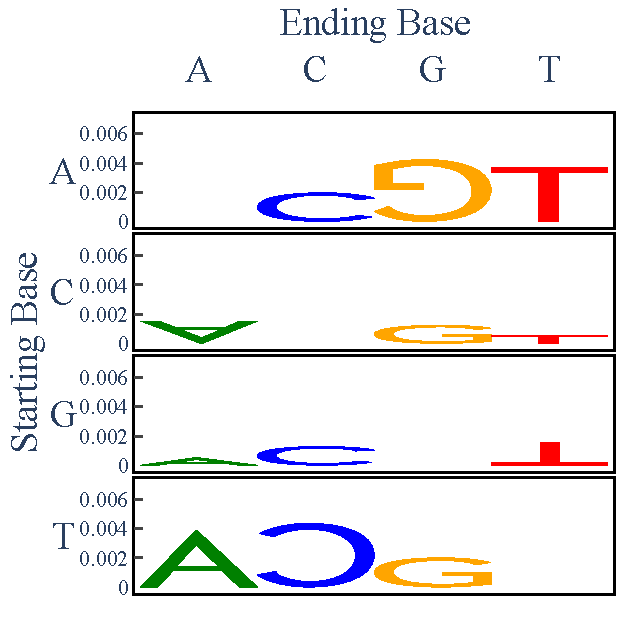
\includegraphics[scale=0.7]{graphics/spectra_Kidney-RCC_Liver-HCC.pdf}
    \caption{Kidney-RCC \textit{v.s.} Liver-HCC}
    \label{fig:spectra_kidney_liver}
    \end{subfigure} \\
    \vspace{0.5cm}
    
    \begin{subfigure}{.5\textwidth}
    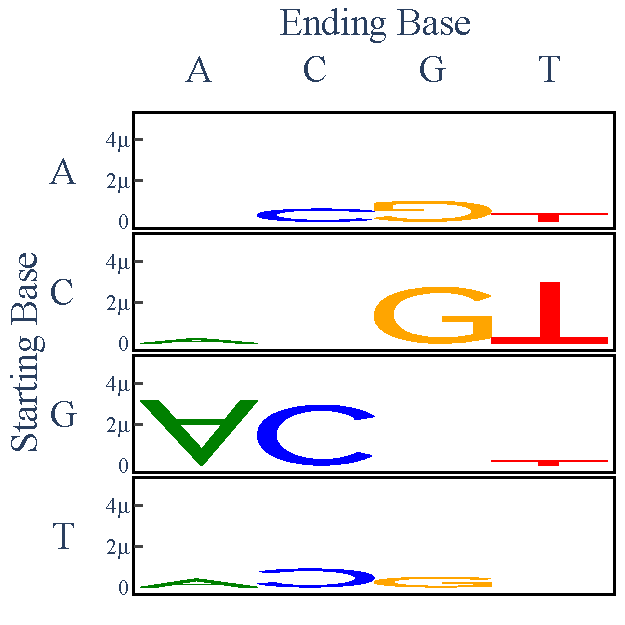
\includegraphics[scale=0.7]{graphics/spectra_CNS-Medullo_CNS-PiloAstro.pdf}
    \caption{CNS-Medullo \textit{v.s.} CNS-PiloAstro}
    \label{fig:spectra_medullo_piloastro}
    \end{subfigure}
    ~
    \begin{subfigure}{.5\textwidth}
    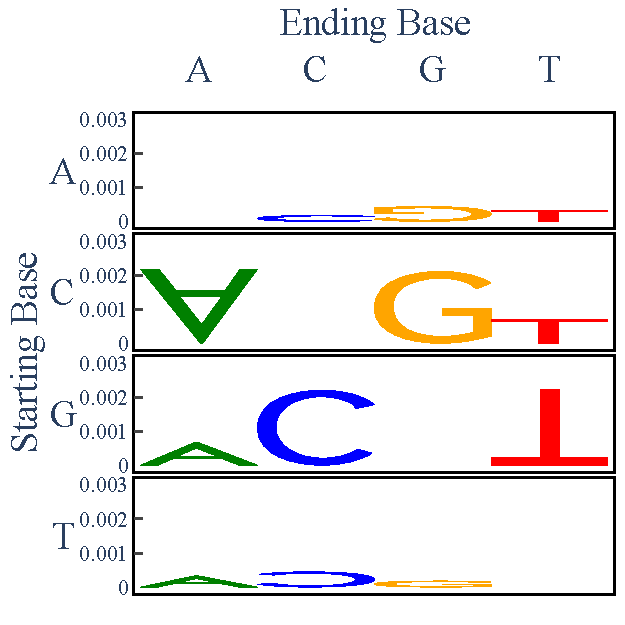
\includegraphics[scale=0.7]{graphics/spectra_CNS-PiloAstro_Lymph-BNHL.pdf}
    \caption{CNS-PiloAstro \textit{v.s.} Lymph-BNHL}
    \label{fig:spectra_piloastro_bnhl}
    \end{subfigure} \\
    \vspace{0.5cm}
\caption{}
    % \caption{\textbf{Base substitutions are promising in discriminating cancers according to $RE$ between cancer pairs.} Similar to Figure \ref{fig:spectra}, for each panel, each row contains the measure of information $RE$ derived from a pair of GLMs. The x-axis is the wildtype base; the y-axis is the product of the substitution. The heights of the letters are $RE$'s. An up-orientation indicates an excess while a down-orientation indicates a deficit of the mutation when comparing the (a) Kidney-RCC to Skin-Melanoma, (b) Kidney-RCC to Liver-HCC, (c) CNS-Medullo to CNS-PiloAstro, (d) CNS-PiloAstro to Lymph-BNHL. More comparisons can be found in Figure \ref{fig:apdx_paired_spectra}.}
    \label{fig:paired_spectra}
\end{figure}

\section{Flanking bases also contain information}

\begin{figure}[ht!]
    \begin{subfigure}{.5\textwidth}
    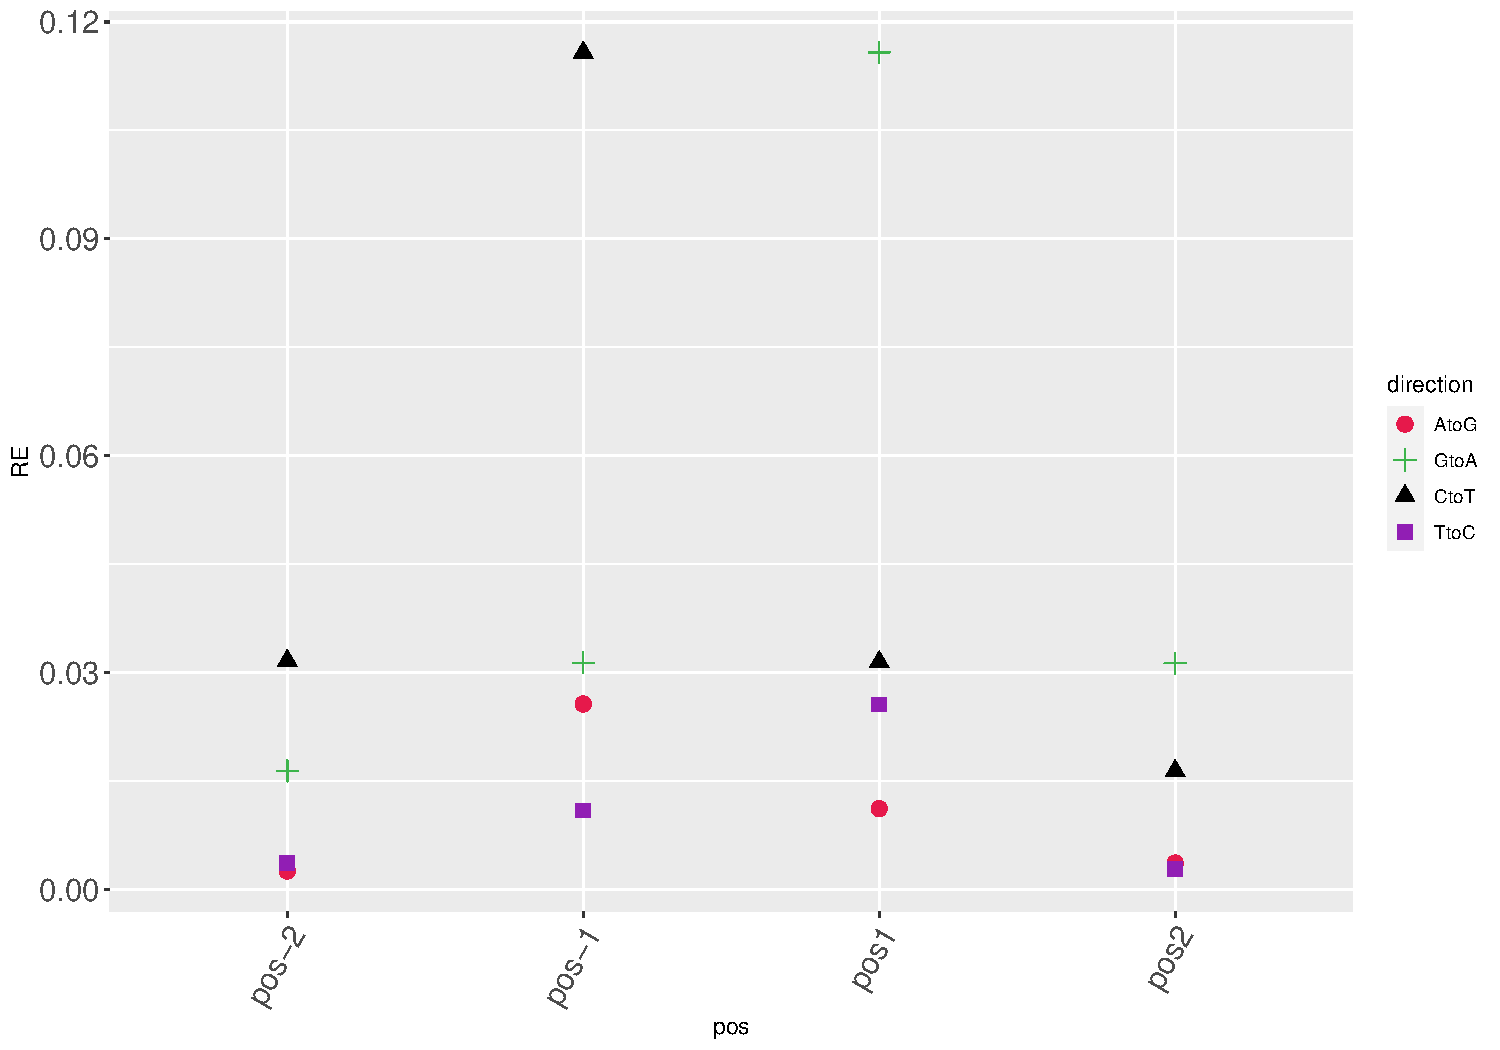
\includegraphics[scale=0.63]{graphics/nbr_transitions_Skin-Melanoma.pdf}
    \caption{transitions/Skin-Melanoma}
    \label{fig:transitions_skin}
    \end{subfigure}
    ~
    \begin{subfigure}{.5\textwidth}
    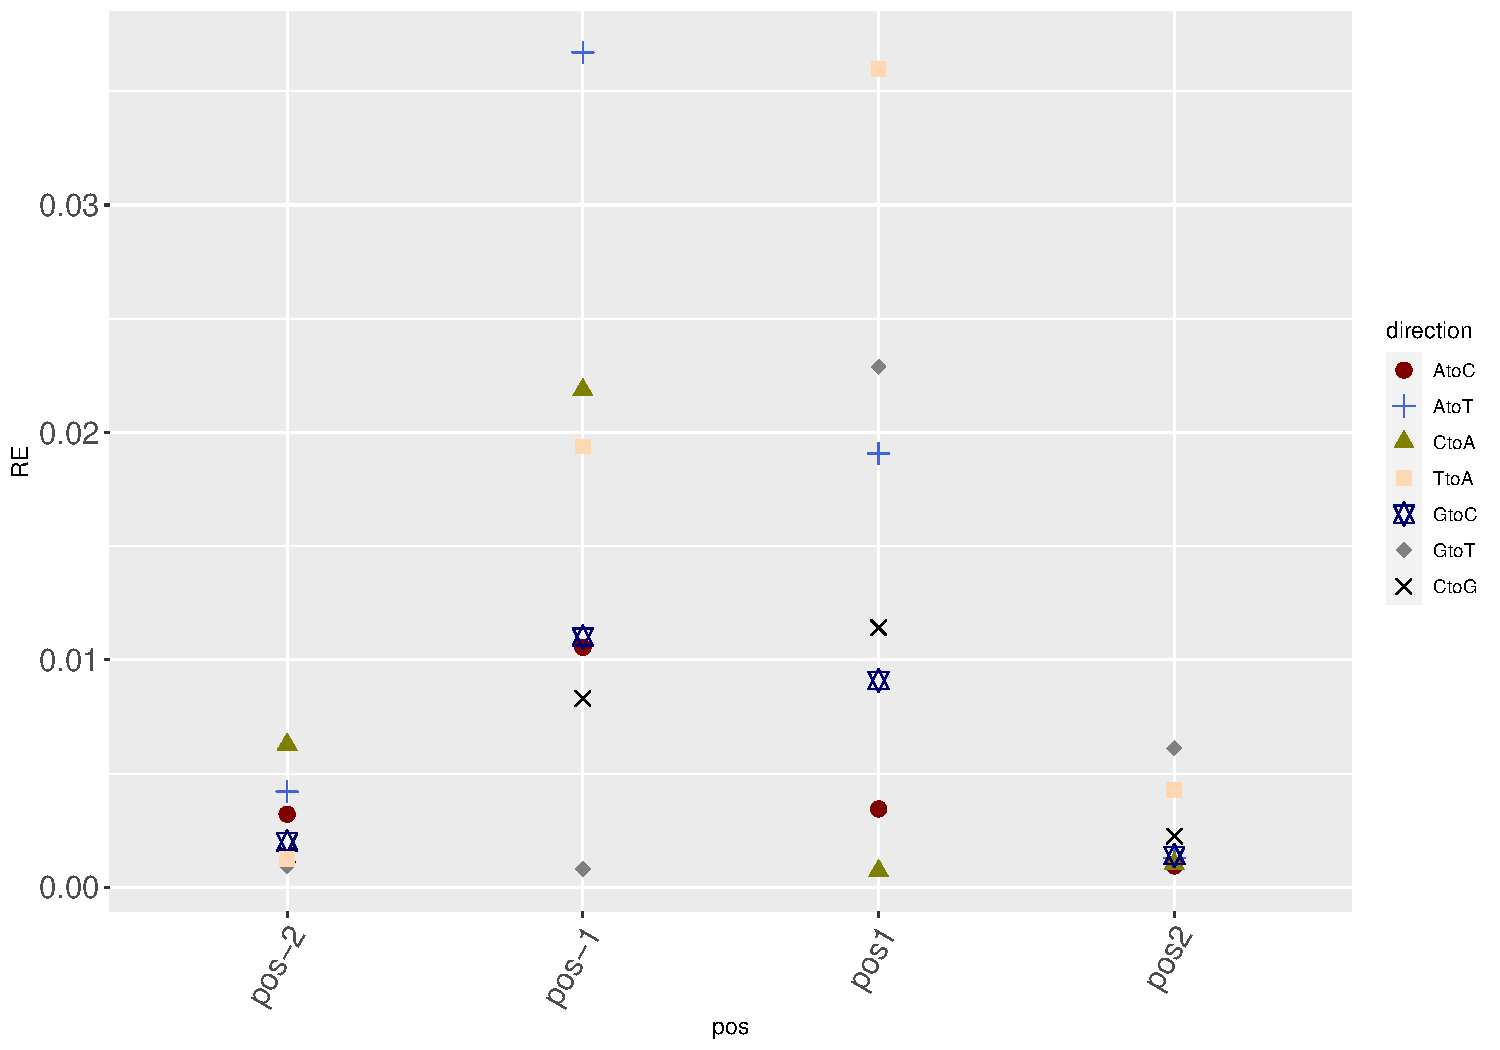
\includegraphics[scale=0.63]{graphics/nbr_transversion_Skin-Melanoma.pdf}
    \caption{transversions/Skin-Melanoma}
    \label{fig:transversions_skin}
    \end{subfigure} \\
    \vspace{0.5cm}
    
    \begin{subfigure}{.5\textwidth}
    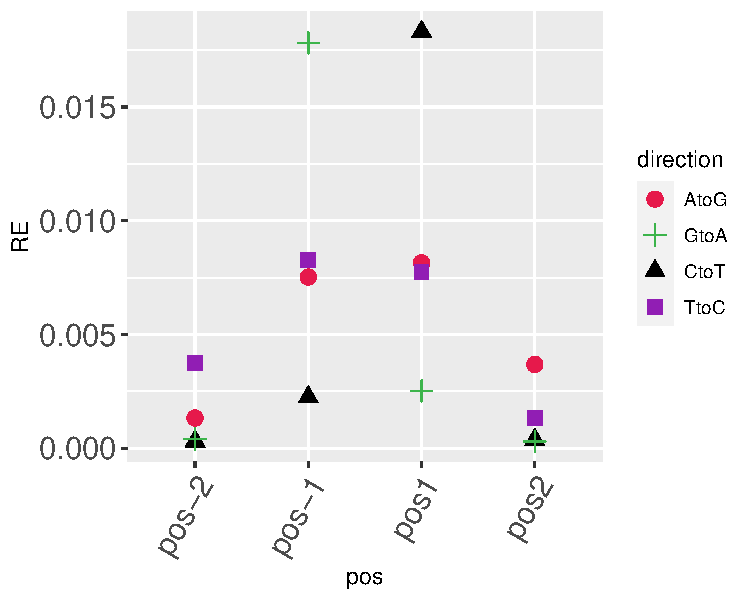
\includegraphics[scale=0.63]{graphics/nbr_transitions_Liver-HCC.pdf}
    \caption{transitions/Liver-HCC}
    \label{fig:transitions_liver}
    \end{subfigure}
    ~
    \begin{subfigure}{.5\textwidth}
    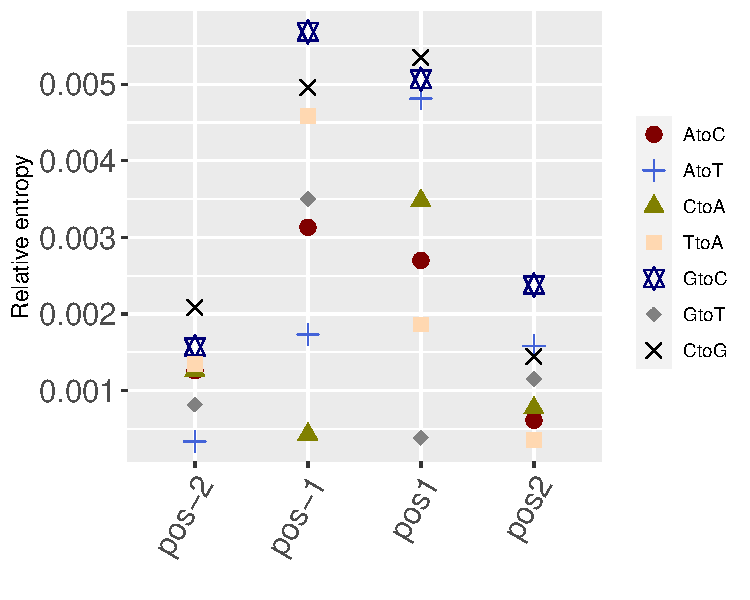
\includegraphics[scale=0.63]{graphics/nbr_transversion_Liver-HCC.pdf}
    \caption{transversion/Liver-HCC}
    \label{fig:transversion_liver}
    \end{subfigure} \\
    
    \caption{\textbf{Flanking bases were a good source of information.} Here, $RE$'s are shown for (a) transitions in Skin-Melanoma (b) transversions in Skin-Melanoma (c) transitions in Liver-HCC (d) transitions in Liver-HCC. The other cancers can be found in Figure \ref{fig:apdx_nbr}. For each panel, each dot was derived from a GLM. The x-axis is the flanking positions with respect to the substitution (substitution at 0); the y-axis is the $RE$ values.}
    \label{fig:nbr}
\end{figure}